%Exercise 4 LaTeX report for TMA 4280
\documentclass[fontsize=11pt,paper=a4,titlepage]{article}
% \usepackage{float} %dunno yet??, probably replaced by amsfonts
\usepackage{listings}
\usepackage[usenames,dvipsnames]{color}		%For the SkyBlue background color for lstlistings
\usepackage{mathtools}
\usepackage{amsfonts,amsmath,amssymb,amsthm}	%For \mathbb
% \usepackage{caption}	%Dunno yet
\usepackage{todonotes}	%For \todo
\usepackage{tabularx}	%for tablecontents wrapping inside cell, instead of cell breaking page width.
\usepackage{verbatim}
\usepackage[margin=3cm]{geometry}

\newcommand*\Laplace{\mathop{}\!\mathbin\bigtriangleup}

\lstset{ %
language=C,							% choose the language of the code
basicstyle=\footnotesize,			% the size of the fonts that are used for the code
numbers=left,						% where to put the line-numbers
numberstyle=\footnotesize,			% the size of the fonts that are used for the line-numbers
stepnumber=1,						% the step between two line-numbers. If it is 1 each line will be numbered
numbersep=5pt,						% how far the line-numbers are from the code
backgroundcolor=\color{SkyBlue},	% choose the background color. You must add \usepackage{color}
showspaces=false,					% show spaces adding particular underscores
showstringspaces=false,				% underline spaces within strings
showtabs=false,						% show tabs within strings adding particular underscores
frame=single,						% adds a frame around the code
tabsize=4,							% sets default tabsize to 4 spaces
captionpos=b,						% sets the caption-position to bottom
breaklines=true,					% sets automatic line breaking
breakatwhitespace=false,			% sets if automatic breaks should only happen at whitespace
escapeinside={\%*}{*)}				% if you want to add a comment within your code
}

\lstset{literate=
	{á}{{\'a}}1 {é}{{\'e}}1 {í}{{\'i}}1 {ó}{{\'o}}1 {ú}{{\'u}}1
	{Á}{{\'A}}1 {É}{{\'E}}1 {Í}{{\'I}}1 {Ó}{{\'O}}1 {Ú}{{\'U}}1
	{à}{{\`a}}1 {è}{{\'e}}1 {ì}{{\`i}}1 {ò}{{\`o}}1 {ù}{{\`u}}1
	{À}{{\`A}}1 {È}{{\'E}}1 {Ì}{{\`I}}1 {Ò}{{\`O}}1 {Ù}{{\`U}}1
	{ä}{{\"a}}1 {ë}{{\"e}}1 {ï}{{\"i}}1 {ö}{{\"o}}1 {ü}{{\"u}}1
	{Ä}{{\"A}}1 {Ë}{{\"E}}1 {Ï}{{\"I}}1 {Ö}{{\"O}}1 {Ü}{{\"U}}1
	{â}{{\^a}}1 {ê}{{\^e}}1 {î}{{\^i}}1 {ô}{{\^o}}1 {û}{{\^u}}1
	{Â}{{\^A}}1 {Ê}{{\^E}}1 {Î}{{\^I}}1 {Ô}{{\^O}}1 {Û}{{\^U}}1
	{œ}{{\oe}}1 {Œ}{{\OE}}1 {æ}{{\ae}}1 {Æ}{{\AE}}1 {ß}{{\ss}}1
	{ç}{{\c c}}1 {Ç}{{\c C}}1 {ø}{{\o}}1 {å}{{\r a}}1 {Å}{{\r A}}1
	{€}{{\EUR}}1 {£}{{\pounds}}1
}
 %config.tex file in same directory

\begin{document}

\begin{center}

% \lstlistoflistings
% \listoffigures
% \listoftables

{\huge Problem set 6}\\[0.5cm]

\textsc{\LARGE TMA4280}\\[0.5cm]
\textsc{\large Introduction to supercomputing -}\\
\textsc{\large Mandatory problem set}\\[0.6cm]

\begin{table}[h]
\centering
\begin{tabular}{ccc}
	\textsc{Christian CHAVEZ} & \textsc{Mireia DUASO} & \textsc{Erlend SIGHOLT}
\end{tabular}
\end{table}

\large{\today}
\vfill
% \section*{Abstract}
\end{center}

\todo[inline]{ABSTRACT}


\clearpage
\section{Introduction}

For the programming code belonging to this problem set, see the $\textit{ex6.c}$
and $\textit{ex6.h}$ files in the zipped archive attached to this hand-in.

For this problem set, we have written our solution in C inspired by the work of
our professor in the subject this problem set belongs to. Hence, our structures,
the general way of thinking, and the algorithms used are based on the work and
lectures done in this subject~\cite{tma4280}.

And as such, a parallelized solver for 2-Dimensional Poisson PDEs is the
objective of this problem set. It is our implementation of this solver we
describe and analyze in this report.


\section{The Poisson problem}
\label{sec:Pois-Prob}

Poisson's equation is an elliptic Partial Differential Equation (PDE) which is
used to model diffusion. It appears in electrostatics, mechanical
engineering, and theoretical physics, among many others.

The problem follows the expression

\begin{eqnarray}
	-\nabla^2 u & = & f \quad \textrm{in} \quad \Omega \\
	u & = & g \quad \textrm{on} \quad \partial\Omega
	\label{eq:Poisson}
\end{eqnarray}

where $f$ is a source function, $g$ is the boundary condition, and $\Omega$ is a
bounded domain.

\section{The Problem Discretized}
\label{sec:Prob-Discr}

We have the below system.

\begin{displaymath}
\begin{bmatrix}
	2 & -1 &  &  &  &  &  \\
	-1 & 2 & -1 &  &  &  &  \\
	 & -1 & 2 & -1 &  &  &  \\
	 &  & \ddots & \ddots & \ddots &  & \\
	 &  &  & -1 & 2 & -1 &  \\
	 &  &  &  & -1 & 2 & -1 \\
	 &  &  &  &  & -1 & 2
\end{bmatrix}
\begin{bmatrix*}[c]
	u_0 \\
	u_1 \\
	u_2 \\
	\vdots \\
	u_{n - 2} \\
	u_{n - 1} \\
	u_n
\end{bmatrix*}
=
\begin{bmatrix*}[c]
	f_0 \\
	f_1 \\
	f_2 \\
	\vdots \\
	f_{n - 2} \\
	f_{n - 1} \\
	f_n
\end{bmatrix*}
\end{displaymath}

Because of the homogeneous boundary conditions, we reduce the problem by $2$
dimensions to become an $(n - 1) \times (n - 1)$ system since $u_0 = u_n = 0$.

\section{The Implemented Solver}

This section is divided into three parts; first we describe our implementation
and analyze its complexity, then we explain how we enabled it to accept smooth
functions, before we finish this section by explaining how we confirmed that our
solver converges towards the correct answer for a given smooth function.

\subsection{Our Implementation}
\label{sec:Impl}

Our implementation is based on the fact and observation that for any Symmetric
Positive Definite (SPD) matrix, we can through the use of a Fast Fourier
Transform (FFT), more specifically the Discrete Sine Transform (DST)
algorithm, implement a solver whose algorithmic FLOP complexity should be
$\textit{O}(n^2log(n))$.

And since TMA4280~\cite{tma4280} is about running mathematical solvers on
super-computing-clusters, we will use the ApplicationProgramInterface (API)
of two libraries; the MessagePassingInterface (MPI) to implement this in
parallel across processes, and OpenMultiProcessing (OpenMP) to parallelize
across threads.

Following, we will describe the dataflow of our implementation, which steps we
intend for it to go through, before analyzing its final FLOP and memory
complexity.

\subsubsection{Implementation Dataflow}
\label{sssec:dataflow}

Our implementation is based on the observation that the following four steps
need to happen in the solver for it to function correctly.

\begin{enumerate}

	\item \label{istep-gen} Generate the $(N - 1)^2$ unknown variables across
	all processes, by creating a matrix $\mathbf{A}$ representing a grid of all
	unknowns, which fills each process with $\sim \frac{N-1}{P \thickspace (=
	Amount 	\thickspace of\thickspace Processes)}$ columns. Assigning each
	gridpoint in $\mathbf{A}$ with a value given by the function we want to
	perform 2-Dimensional Poisson operation on (which is given the $i$th and
	$j$th position as input) multiplied with step-length between our grid points
	due to the discretization of the 2D Poisson problem, e.g. $h^2, \thickspace
	h = \frac{1}{n}$.

	\item \label{istep-fst1} Use the Fourier Sine Transform (FST) on each
	coloumn of the matrix within each process, thereby Fourier transforming the
	whole matrix, before transposing it across all processes (let us call the
	transposed matrix $\mathbf{B}$). The transposition requires one ``round
	of communication'' across all processes, before an inverse FST is performed
	on $\mathbf{B}$.

	\item \label{istep-tens} Perform the tensor operation based on the
	five-point stencile given from the 2D nature of the Poisson operation on
	each element $b_{ij}$ by dividing each element on its corresponding sum of
	the terms $d_i + d_j$, which are the respective eigenvalues of the matrix $
	\mathbf{A}$.

	\item \label{istep-fst2} Repeat step~\ref{istep-fst1}, except now perform
	the FST on $\mathbf{B}$, transpose it back to $\mathbf{A}$, and perform the
	inverse FST on $\mathbf{A}$. $\mathbf{A}$ (spread across all $P$ processes
	used) now represents the solution found to the function inputted in
	step~\ref{istep-gen}.

\end{enumerate}

The parallelization is achieved by splitting the matrix $\mathbf{A}$'s columns
across the processes used with the MPI API. Since the functions that perform the
FST are not parallelization, and they need to perform the transformation on a
whole column at the time, these can be parallelized by using OpenMP, running
several concurrent threads.

This division of labor fits well with the implementation, since the OpenMP tasks
can share memory, and the MPI ones should not (hence the need for its own memory
as naturally befits a process vs. a thread).

\subsubsection{Implementation Complexity}

The complexity of our implementation can be described as following with the help
of the list in subsection~\ref{sssec:dataflow}.

In the following subsection, $n$ is the input size given as parameter to the
solver).

\paragraph{The Complexity of Step~\ref{istep-gen}} comes from the following
actions the solver performs in this step.

It generates the data structures with which the solver performs the 2D Poisson
operation. Hence, in step~\ref{istep-gen}, the following data structures are
created with the following operations inside of each process;

\begin{itemize}
	\item The ``work-matrix'', which we called $\mathbf{A}$ in
	step~\ref{istep-gen}, will have $k = \frac{(N-1)}{P}$ columns, which each
	have $N-1$ rows, giving a total size to matrix; $ProcSize = k\cdot(N-1)$.
	To initialize each of the matrix variables with values, the run-time
	complexity is a constant. Thus, for initializing matrix $\mathbf{A}$, it
	requires $\textit{O}(ProcSize)\Rightarrow \textit{O}(n^2)$ run-time
	complexity and memory. (Since more often than not, $P \ll N$, the complexity
	is simplified from being $\textit{O}(\frac{(N-1)^2}{P})$, to $\it
	{O}(n^2\times \frac{1-\frac{2}{n}+\frac{1}{n^2}}{P})$, and finally into
	$\textit{O}(n^2)$).

	\item The ``transpose matrix'', called $\mathbf{B}$ in
	step~\ref{istep-fst1}, is identical in size and run-time complexity when
	comparing with matrix $\mathbf{A}$; $\textit{O}(n^2)$. This one is also
	initialized in step~\ref{istep-gen}.

	\item The ``eigenvalue vector'', mentioned in step~\ref{istep-tens}, is a
	vector containing the eigenvalues for the 2D Poisson problem. As such they
	are not dependent on the function the solver performs on (the \emph{f}
	function, if you will). Its complexity in run-time will be constant, once
	for each variable; $\textit{O}(N-1)$, while the memory depends as hinted
	by the run-time complexity on the input size. And since the vector is $N-1$
	elements long, the memory complexity will also be $\textit{O}(N-1)$.
	In other words, $\textit{O}(N)$.

	\item There are several other help-variables used, but these are not
	dependent on the problem size input $N$, and will hence not incur any
	greater complexity beyond a constant $C$ added, like $\textit{O}(f(n) + C)$
	Which again can be simplified into $\Rightarrow \textit{O}(n^2)$.
\end{itemize}

\paragraph{The Complexity of Step~\ref{istep-fst1}} comes from the from the
Fourier Transforms and the transpose operation we perform on the $\mathbf{A}$
matrix.

There are three operations performed in this step; a Fourier transform on each
column of $\mathbf{A}$, a transpose of $\mathbf{A}$ (and it is now we start
referring to the transposed matrix as $\mathbf{B}$), and then an inverse Fourier
transform on each of column of $\mathbf{B}$.

Below we will detail the complexity for each of these three steps, considering a
single process;

\begin{itemize}
	\item The first FST operation is performed on each column of $\mathbf{A}$
	present in the process, let us call this number $k$ like in the previous
	step complexity analysis. Since the FST requires $\textit{O}(k(n-1)
	(n-1)log(n-1))$, which simplified turn into $\textit{O}(n^2
	log(n))$. Memory complexity however, is not \textit{O}$(n^2log(n)
	)$. The FST requires an extra ``work-space'' in which to store temporary
	variables which represent the inputted ones. But it needs not only to store
	two duplicates, but also to store their complex values, resulting into {\it
	O}$(4k\cdot(n-1)) \Rightarrow$ \textit{O}$(n)$.

	\item The transpose operation is performed on the matrix as a whole, across
	all processes, and requires an iteration over each element in matrix $
	\mathbf{B}$. Hence, since the transpose needs to re-order the elements
	twice, once before sending, and once after, the complexity of this operation
	ends up as \textit{O}$(3(n-1)^2)$. This in turn can be simplified into
	\textit{O}$(n^2)$. There is no added memory complexity needed for the transpose.

	\item The inverse FST is identical to the regular FST in terms of complexity
	both for run-time and memory.
\end{itemize}

\paragraph{The Complexity of Step~\ref{istep-tens}} is smaller than the other
steps, since in this step only involved one new data element requiring storage,
the vector containing the eigenvalues of $\mathbf{A}$, of which there are {\it
O}$(n-1)$.

Run-time complexity is constant per element, and we need to traverse all
elements in $\mathbf{B}$ (which represents $mathbf{A}$ transposed), per process.
Hence, the run-time complexity becomes \textit{O}$(n^2)$ for a serial
implementation, but \textit{O}$(\frac{n^2}{T\thickspace (=Amount\thickspace of
\thickspace threads)})$ for our implemented solver.

\paragraph{The Complexity of Step~\ref{istep-fst2}} is identical to the
complexity of step~\ref{istep-fst1} in terms of run-time, namely \textit{O}$(n^2
log(n) + n^2 + n^2log(n) = $\textit{O}$(n^2\cdot
log(n))$. Memory complexity however becomes only \textit{O}$(Cn^2)$ where $
C$ is a constant offset, dependent only on the amount of processes and threads
the solver utilizes.

\paragraph{The Total Complexity} then becomes as following for our
implementation:

\begin{itemize}
	\item Memory: \textit{O}$(n^2)$
	\item Run-time: \textit{O}$(n^2log(n))$
\end{itemize}

%section (e)
\subsection{Accepting Smooth Functions}

We are asked to enable our implemented solver to accept smooth functions, by
changing the initial values we give the grid points in the above mentioned matrix
$\mathbf{A}$. We chose to test this with the function given in the problem
text's appendix \textit{B}, namely $f(x,y) = 5\pi^2 sin(\pi x) sin(2\pi y)$.

The function our implemented solver performs the 2D Poisson operation on has to
be hard coded into the code. Hence, the smooth function we use (and the code we
use to check its correctness with), is hard coded into the program. If, at any
point, it is desired that the solver performs the Poisson 2D operation on any
other function, that function would also have to be hard coded into our
implementation.

For each process' $\mathbf{A}$ to know which values it needs to initialize with,
since that depends on what part of the grid this $\mathbf{A}$ represents, all
processes have an array which stores the \textit{offset} of which each column of
the grid point said process' $\mathbf{A}$ starts representing.

\subsection{Correctness Convergence}

To confirm that our solver actually returns a grid of values representing the
correct values for the function ``solved'',

\todo[inline]{Decide if we make another section, to analyze and report
communication, FLOP, FLOPS, and so on...}

\section{Results}

In this section we present the runtime-results of our solution.

We have tested the different parallelizations of our solution separately, in
order to analyze their contribution to the solution as a whole, as well as the
whole solution in itself.

\subsection{MPI Results}

In order to test the MPI-implementation we have tested on selected amounts of
processors and nodes, to test both the MPI-implementation effectiveness, and the
communication delay between nodes.

\subsubsection{Single Node}

First we tested the program on only one node on the Kongull-cluster. Seeing as
one node may use up to 12 processors, we elected to test with that, as well as
selected increments below that.

As is shown in the figure below, the MPI-implementation of the
solution can in itself be considered successful, seeing as it is almost
perfectly parallel with runtime decreasing linearly with respect to the amount
of processors added. The runtime with 8 processors is just about half of that
with 4, and similarly with 12 and 6 processors.

\hspace*{-1.7cm}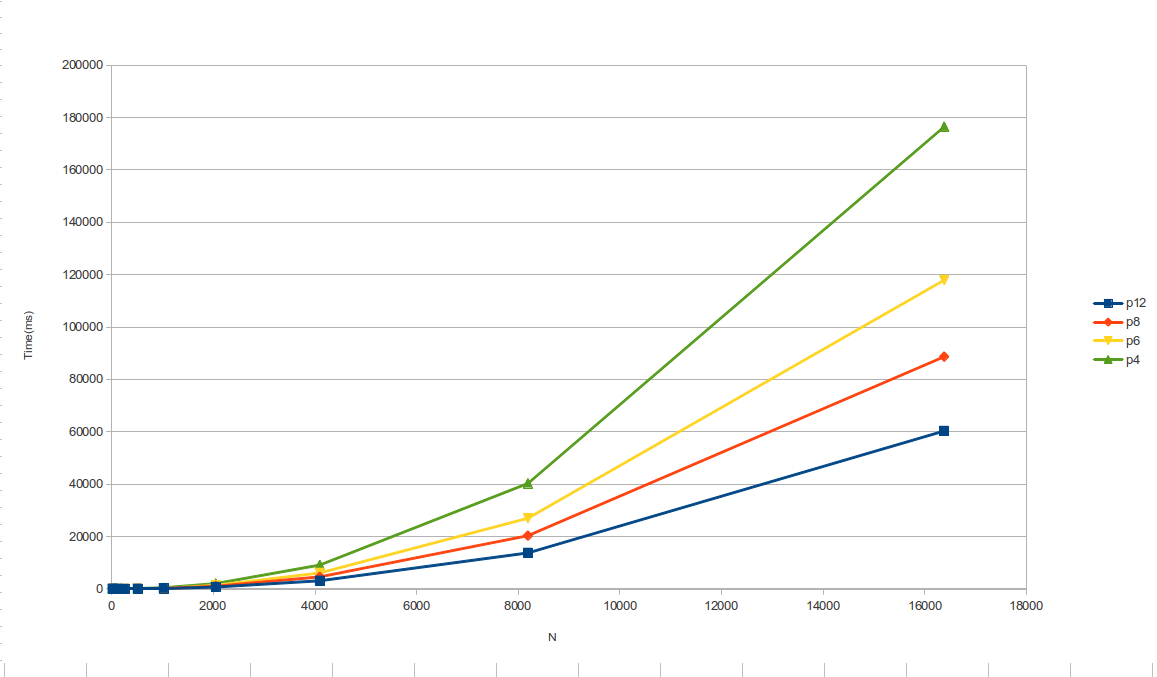
\includegraphics[scale=0.6]{pics/pX.png}

\subsubsection{Multiple Nodes}

Next we examined the communication costs across several nodes on Kongull. In
order to do this we ran several jobs with a total of 36 processes divided across
varying amounts of nodes.

If the communication costs across nodes were negligible, we would expect to see
a runtime of approximately \emph{20000 ms}, seeing as that would constitute an
improvement in runtime by a factor of 3 with a multiplication in the amount of
processes by 3. This in comparison to the runtime with 12 processes on a single
node \emph{(60000 ms)}, as shown in the previous section.

We did not see a linear decrease in runtime, as can be observed in the figure
on the next page where the run-times of 36 processes divided by 3, 6, and 9, can
be seen.

One can observe that the runtime approaches the ideal linear increase of
\emph{20000 ms} as the amount of nodes the problem is divided across increases.
This leads us to believe that the limiting factor in achieving linear speedup in
the parallelization is the communication bandwidth between nodes. Each node
receives a part of the whole problem which is in proportion to its amount of
processes, and this means that when the 36 processes are divided across fewer
nodes, each node receive a larger part. This, in turn, means that more data has
to be sent each time the processes communicate, something which obviously takes
more time than sending less to more nodes on this architecture.


While the data for smaller problem sizes is cluttered with noise, we can clearly
see from the plot that the bandwidth starts to limit the parallelization around
$n = 2^{13}$, and that adding more nodes past this point clearly is beneficial
to the parallelization efficiency. One could expect that as the problem size
increases past the scope we have tested on, one could see several more such
points, where dividing across 9 nodes as we have done at the most in our testing
would also start seeing falloff in parallel efficiency as it would have to send
too much data between each of the nodes.

\hspace*{-1.5cm}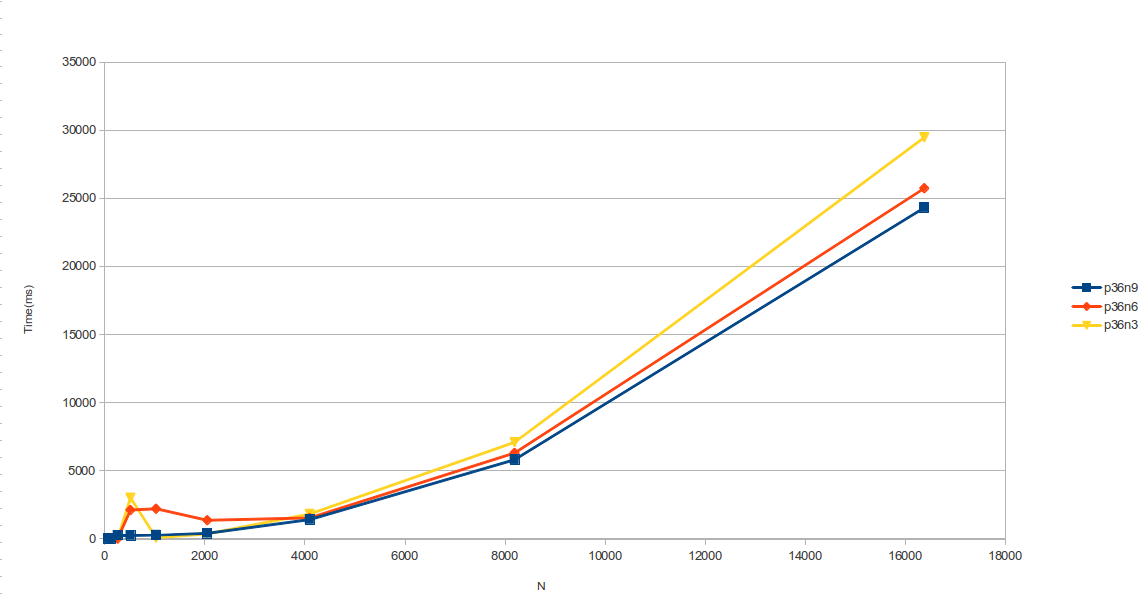
\includegraphics[scale=0.6]{pics/p36nX.png}

\subsection{OpenMP Results}

When it came to testing the OpenMP speedup, we were more limited by what we
could test, due to being limited to a single node on Kongull, and thus a maximum
of 12 threads. Below is a plot of the timing, which shows that while OpenMP in
itself grants a decent speedup, it is inferior to MPI by itself. OpenMP by
itself is not of much interest however, seeing as it cannot make use of more
than one node on Kongull, and therefore is limited to adding a maximum of 12
threads. In the next section however, we will look at how it performs in concert
with MPI.

\hspace*{-1.7cm}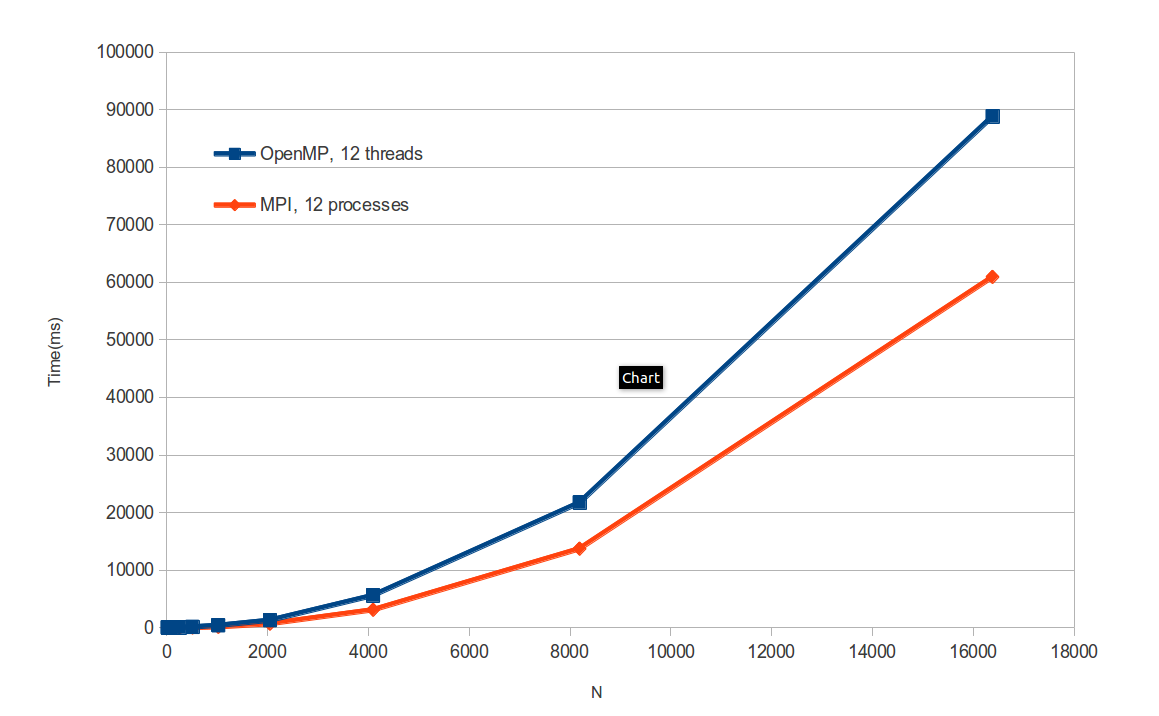
\includegraphics[scale=0.6]{pics/omp.png}

\subsection{Combined Results}
\subsubsection{The Data}

For testing the combined implementation of both OpenMP- and MPI-parallelization
we used the same amount of nodes and processes as in the MPI test. The MPI test
was done with one thread per process and 36 processes total, which gives $p*t =
36*1 = 36$. Here we also tested with various combinations of $p*t=36$, and with
3, 6, and 9 nodes, for good comparison. The legend on this plot is slightly
different from the MPI one, where its \emph{p(rosessor per node)t(hreads per
node)n(odes)}, so one multiplies them together to get a total of 36 for each
case.

\hspace*{-2.3cm}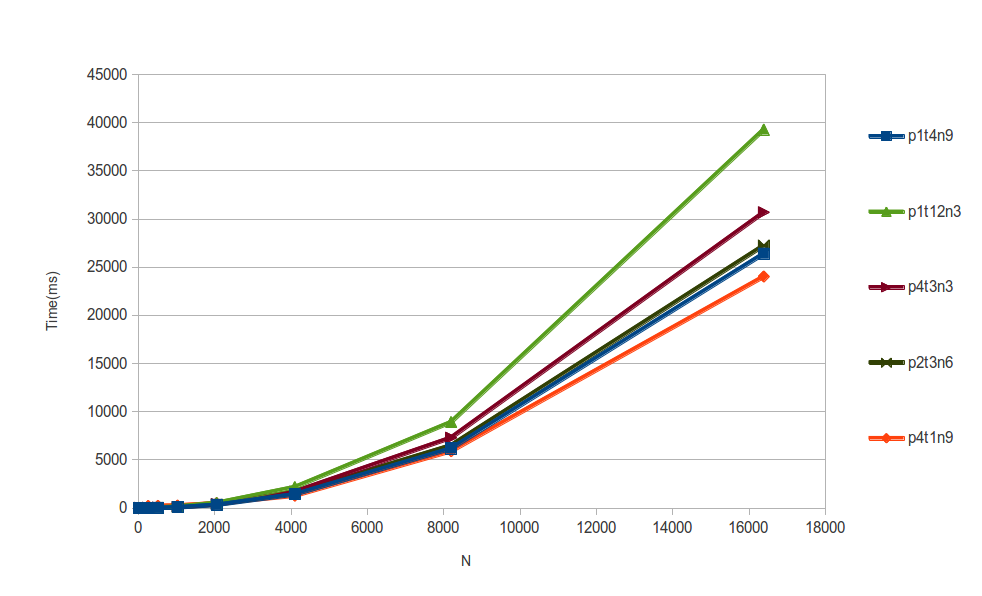
\includegraphics[scale=0.73]{pics/plot.png}

It is clearly visible that dividing just the threads over several nodes, as in
$p1t12n3$, is not the most effective parallelization strategy. It behaves like
the pure OpenMP implementation does in relation to the pure MPI implementation.
One can observe the same in the test cases: One process and several threads
performs worse than the opposite, or a mix of several of each.

One can also observe that if one ignores the test-cases where one processor per
node was used, the performance for each node amount is about the same as in the
pure MPI-case. This indicates that the node amount is quite significant in terms
of parallel efficiency as the problem size grows, something which strongly
implicates the communication bandwidth between nodes as a major limiting factor,
as previously discussed in the MPI-result section.

In addition to this it should be said that $p2t2n9$ behaved exactly like the
p4t1n9 shown in the plot, and the same goes for $p3t2n6$ in relation to
$p2t3n6$. From this we can conclude that as long as one avoids using just one
processor per node, the combined implementation is about equivalent with the
pure MPI implementation, but if you do use just one processor per node, it is
worse.

\subsubsection{Conclusions From Results}

By testing the combined implementation of MPI and OpenMP, we have learned that
if certain configurations are avoided, it may be desirable to use both
parallelization technique seeing as it does not perform any worse than only MPI.
The possible benefit of using both comes from the ability to better utilize all
processors on a node when dividing a certain amount of processes across nodes.
Any leftover processors on a node can then be utilized to add additional threads
to solve the problem on each node, without affecting any specific desired
processor division.

We have not tested this assumption to a sufficiently large degree, and it might
therefore be desirable to do more extensive testing, but we believe it is safe
to say that such a solution probably is the most flexible one, assuming one has
the time to implement both. However, should one only have time to implement one
solution, the OpenMP one is decidedly faster, while the MPI one provides for a
better level of parallelization.

\subsection{Scaling and Complexity} When it comes to scaling, we are of course
also interested in how the results scale to the computational complexity of the
problem. Solving the problem with the DST takes $\it O (n^2log(n))$ floating point
operations, and it is therefore important to compare the implementation to this,
in order to see how the algorithm implementation compares to the theory.

Below is a plot comparing the timing results from 36 processors, with an
$n^2log(n)$ plot of the problems input size. (The $n^2log(n)$ plot is divided by
a costant to improve the plot, seeing as constants are inconsequential anyway).

\hspace*{-1cm}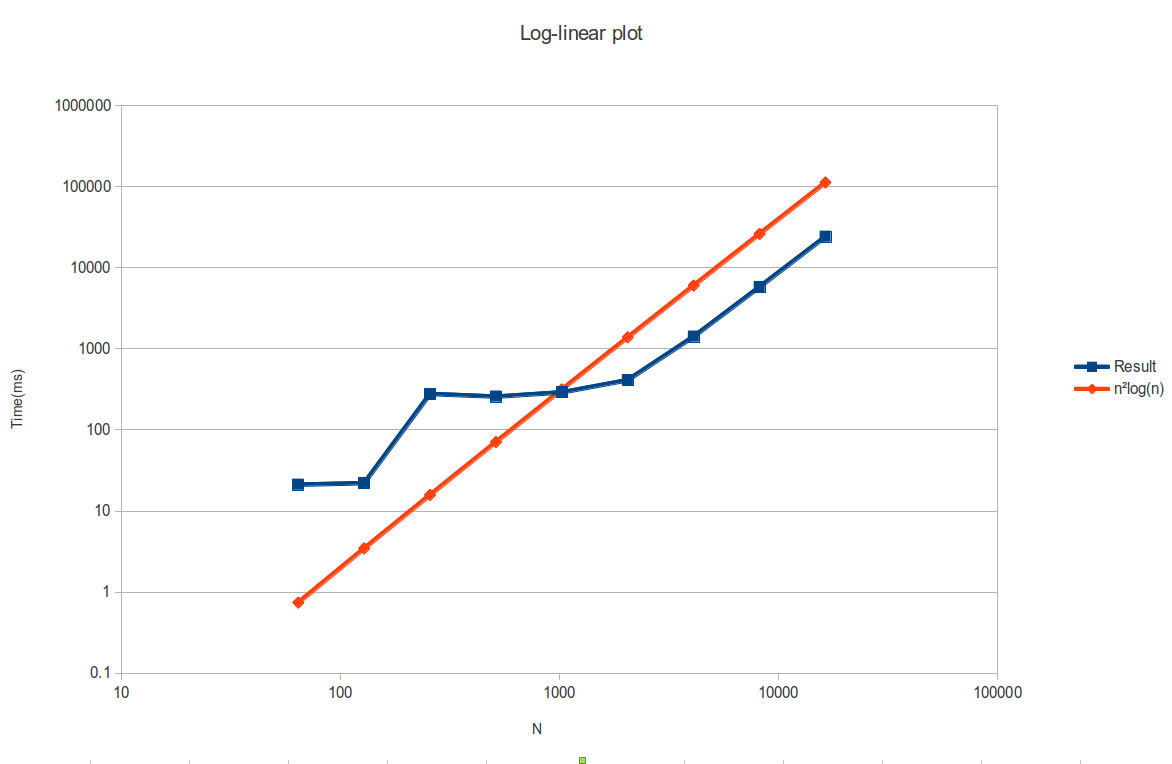
\includegraphics[scale=0.55]{pics/logplot.png}

We can see that for $n > 1024$ they scale identically, while below this point
there are some differences. Most of this, however, should be explainable by
noise in our data, as well as startup-costs of the program. Other than that,
this is as should be expected, and indicates that the implementation is correct
as far as complexity is concerned.

% (f)
\section{Non-Homogeneous Dirichlet Boundary Conditions}

We want to know which part of our code has to be modified if we change the
original problem, when $u \neq 0$ on $\partial\Omega$, and $\Omega = (0,1)
\times (0,1)$.

In the analytic case, to tackle the new problem we define $v$ as a new solution,

\begin{equation}
	v = u - g
\end{equation}

for some lifting function $g$. In the newly defined solution, $g$ is supposed to
set the values of $v$ along the boundaries to $0$.

If we want our code to solve the problem with these new conditions, we need to
transform the original problem into

\begin{displaymath}
	\mathbf{A} \times (\mathbf{u} + \mathbf{u_B}) = h^2 \mathbf{f}
\end{displaymath}

where $\mathbf{A}$ will be a $(n + 1) \times (n + 1)$ matrix, $\mathbf{u}$ will
be the old solution, $\mathbf{f}$ the source, $h$ the length of the step, and
$\mathbf{u_B}$ the function that satisfies the boundary conditions.

Considering the discretization of the original problem in section~\ref{sec:Prob-
Discr}, if we re-compute the left hand-side of that system, we get

\begin{displaymath}
\begin{bmatrix}
	2u_0 - u_1 \\
	- u_0 + 2u_1 - u_2 \\
	- u_1 + 2u_2 - u_3 \\
	\vdots \\
	- u_{n - 3} + 2u_{n - 2} - u_{n - 1} \\
	- u_{n - 2} + 2u_{n - 1} - u_{n} \\
	- u_{n - 1} + 2u_n
\end{bmatrix}
=
\begin{bmatrix*}[c]
	f_0 \\
	f_1 \\
	f_2 \\
	\vdots \\
	f_{n - 2} \\
	f_{n - 1} \\
	f_n
\end{bmatrix*}.
\end{displaymath}

but this system is redundant since there are $n - 1$ variables, and $n + 1$
equations. Hence, we can remove the first and the last terms, and we only need
to add a vector to our previous matrix.

Then the system will be written as

\begin{displaymath}
\begin{bmatrix}
	2 & -1 &  &  &  &  &  \\
	-1 & 2 & -1 &  &  &  &  \\
	 &  & \ddots & \ddots & \ddots &  & \\
	 &  &  &  & -1 & 2 & -1 \\
	 &  &  &  &  & -1 & 2
\end{bmatrix}
\begin{bmatrix*}[c]
	u_1 \\
	u_2 \\
	\vdots \\
	u_{n - 2} \\
	u_{n - 1}
\end{bmatrix*}
+ \begin{bmatrix*}[c]
	- u_0 \\
	0 \\
	\vdots \\
	0 \\
	- u_n
\end{bmatrix*}
=
\begin{bmatrix*}[c]
	f_1 \\
	f_2 \\
	\vdots \\
	f_{n - 2} \\
	f_{n - 1}
\end{bmatrix*}.
\end{displaymath}

\section{Handling Different Domains}
%(g)

If we consider the geometry of the domain, we may want to solve the
PDE~\ref{eq:Poisson} in a rectangle $\Omega = (0, L_x) \times (0, L_y)$. To
accomplish this, we need to declare two lengths instead of our old $h$. Namely,
$h_x$ and $h_y$, which would have the same value if we considered a square, and
different values than we would get working with a rectangle.

Following the diagonalization shown in the lectures, the only change that needs
to be implemented is the following.

In the implemented tensor-operation, instead of simply summing the two
eigenvalues whose sum we divide the variable with, we need to divide each
eigenvalue with their corresponding step-lengths of the finite grid, $h_x^2$ and
$h_y^2$. This is due to the fact that we do not store our step-lengths in the
source function.

\section{Conclusion}

We can conclude from our results, that parallelization of a DST-based solver for
the Poisson problem is an excellent way to improve performance and enable
solving of larger problem sizes. We have also learned that a distributed
solution can be limited in its parallel efficiency by communication bandwidth
between different nodes in a distributed architecture, when the problem size
grows large enough, as seems to be the case on the Kongull system.

We have also observed that a combined solution of MPI and OpenMP offers the
largest amount of flexibility, at no downsides other than more time required to
implement and test it, while solutions with just MPI or OpenMP has downsides
compared to each other. The MPI solution takes considerably more time to
implement and test, but offers the superior speedup and parallelization degree.
While on the other hand OpenMP-support is very fast to implement, but offers a
significantly worse speedup compared to MPI.

\todo[inline]{Summarize the best/worst results of the result chapter. Also
repeat what we can and cannot to do from Mireia's math-section.}



\bibliography{bibliography}{}
\bibliographystyle{plain}

\end{document}
